
\section{Dispersal model: basic reproduction number}

As remarked in the opening chapters, the basic reproduction number is widely used in the %
study of epidemics in human and animal populations. %
The $R_0$ value is fundamental to understand the threshold of transmission, if $R_0>1$ the %
disease will spread through the population, or otherwise die out. The concept of $R_0$ is %
widely used, and misinterpreted \cite{delamater2019complexity}, and many different ways of %
calculating $R_0$ and available \cite{perspectives-on-r0}.\\

Various studies have considered $R_0$ for plant-based diseases %
\cite{gubbins2000population, park2001invasion, doi:10.1146/annurev.phyto.011108.135838, van2011periodic, mikaberidze2016invasiveness}. %
However, in the context of tree and plant-based epidemiology the concept remains far less %
explored. In general, $R_0$ is a complicated parameter which may vary in response to abiotic %
factors, such as temperature, humidity and wind-speed, or a changing contact network. %
When defining an $R_0$ value for tree-disease, the importance of spatial structure cannot be %
ignored \cite{park2001invasion}.\\

At the small scale we have a uniformly structured population. %
However, for larger scales there is considerable spatial heterogeneity. %
There fore, it is expected that some regions above the threshold host-density can support %
local reproduction of the pathogen, while some regions below the density-threshold cannot. %
Importantly, any measure of $R_0$ should separate these regimes with the threshold $R_0>1$. %
Infected regions are therefore likely to be `\textit{patchily}', distributed among the host %
population \cite{park2001invasion}.\\

Defining an informative $R_0$-value for tree-based pathosystems is far from simple. %
In particular, the value of $R_0$ will likely depend on the spatial scale we choose to %
consider \cite{mikaberidze2016invasiveness}. %
If  $R_0$ is measured over a small domain, we would under-count the number of secondary %
infections because long-range dispersal could infect a non-trivial amount of trees in %
neighbouring domains. %
Furthermore, a spatially-structured host population with dispersal-mediated interactions %
can expect to violate the \textit{well-mixed} population assumption\footnote{A spatially-dependant dispersal mechanism will limit the contact network and prevent the host population from being well-mixed}. 
Therefore care is needed in deciding how to define $R_0$.\\

\chapter{A non-local dispersal model}
\label{ch5:dispersal-model}

\subsection{Contact-tracing $R_0$}

An analytical solution to $R_0$ was presented previously in \textcolor{red}{CHAPTER 4}. %
In that approach, tertiary ($3^{rd}$ order generation) infections were not permitted. %
This allowed us to solely count the number of secondary infected trees due to the source infection. %
This is likely to over-estimate the number of secondary infections an infected tree could produce. %
Here, an alternate definition is presented that incorporates the effect of tertiary infections %
(up to $n^{th}$ order)  on the spatial structure.\\

Figure \ref{fig:contact-trace}(a) depicts a method, by computational means, of collecting $R_0$ %
through contact-tracing tree-to-tree interactions. %
At $t=0$ the primary infected tree, denoted by $A$, produces three $2^{nd}$ order infections %
$B$-$D$ shown in orange. %
The proceeding $3^{rd}$ order infections are shown in green, that is, $B$ infects $E$ and $F$ while $C$ infects $G$. %
Over the course of a simulation, the mean number of secondary infections produced by an $n^{nth}$ order infected tree is found. %
Doing so, leads to a generational mean denoted by $R^i_0$, an in this particular scenario $R^2_0=3$ and $R^3_0=1$. 
Throughout a simulation, a record is kept of all infection histories i.e. which tree infects which. 
To achieve this, trees are treated as particles in the sense that individual interactions between them are computed. 
This can be seen as equivalent to contact-tracing the resulting epidemic \cite{eames2003contact}. \\

For the remainder of this thesis, the basic reproduction number will be defined as $R_0=R^2_0$ unless otherwise stated. 
Defining $R_0$ in this way extends the previous definition to account for the realistic %
saturation around the primary infected trees neighbourhood. This gives an improved measure %
of the threshold for invasion.\\

\begin{figure}
    \centering
    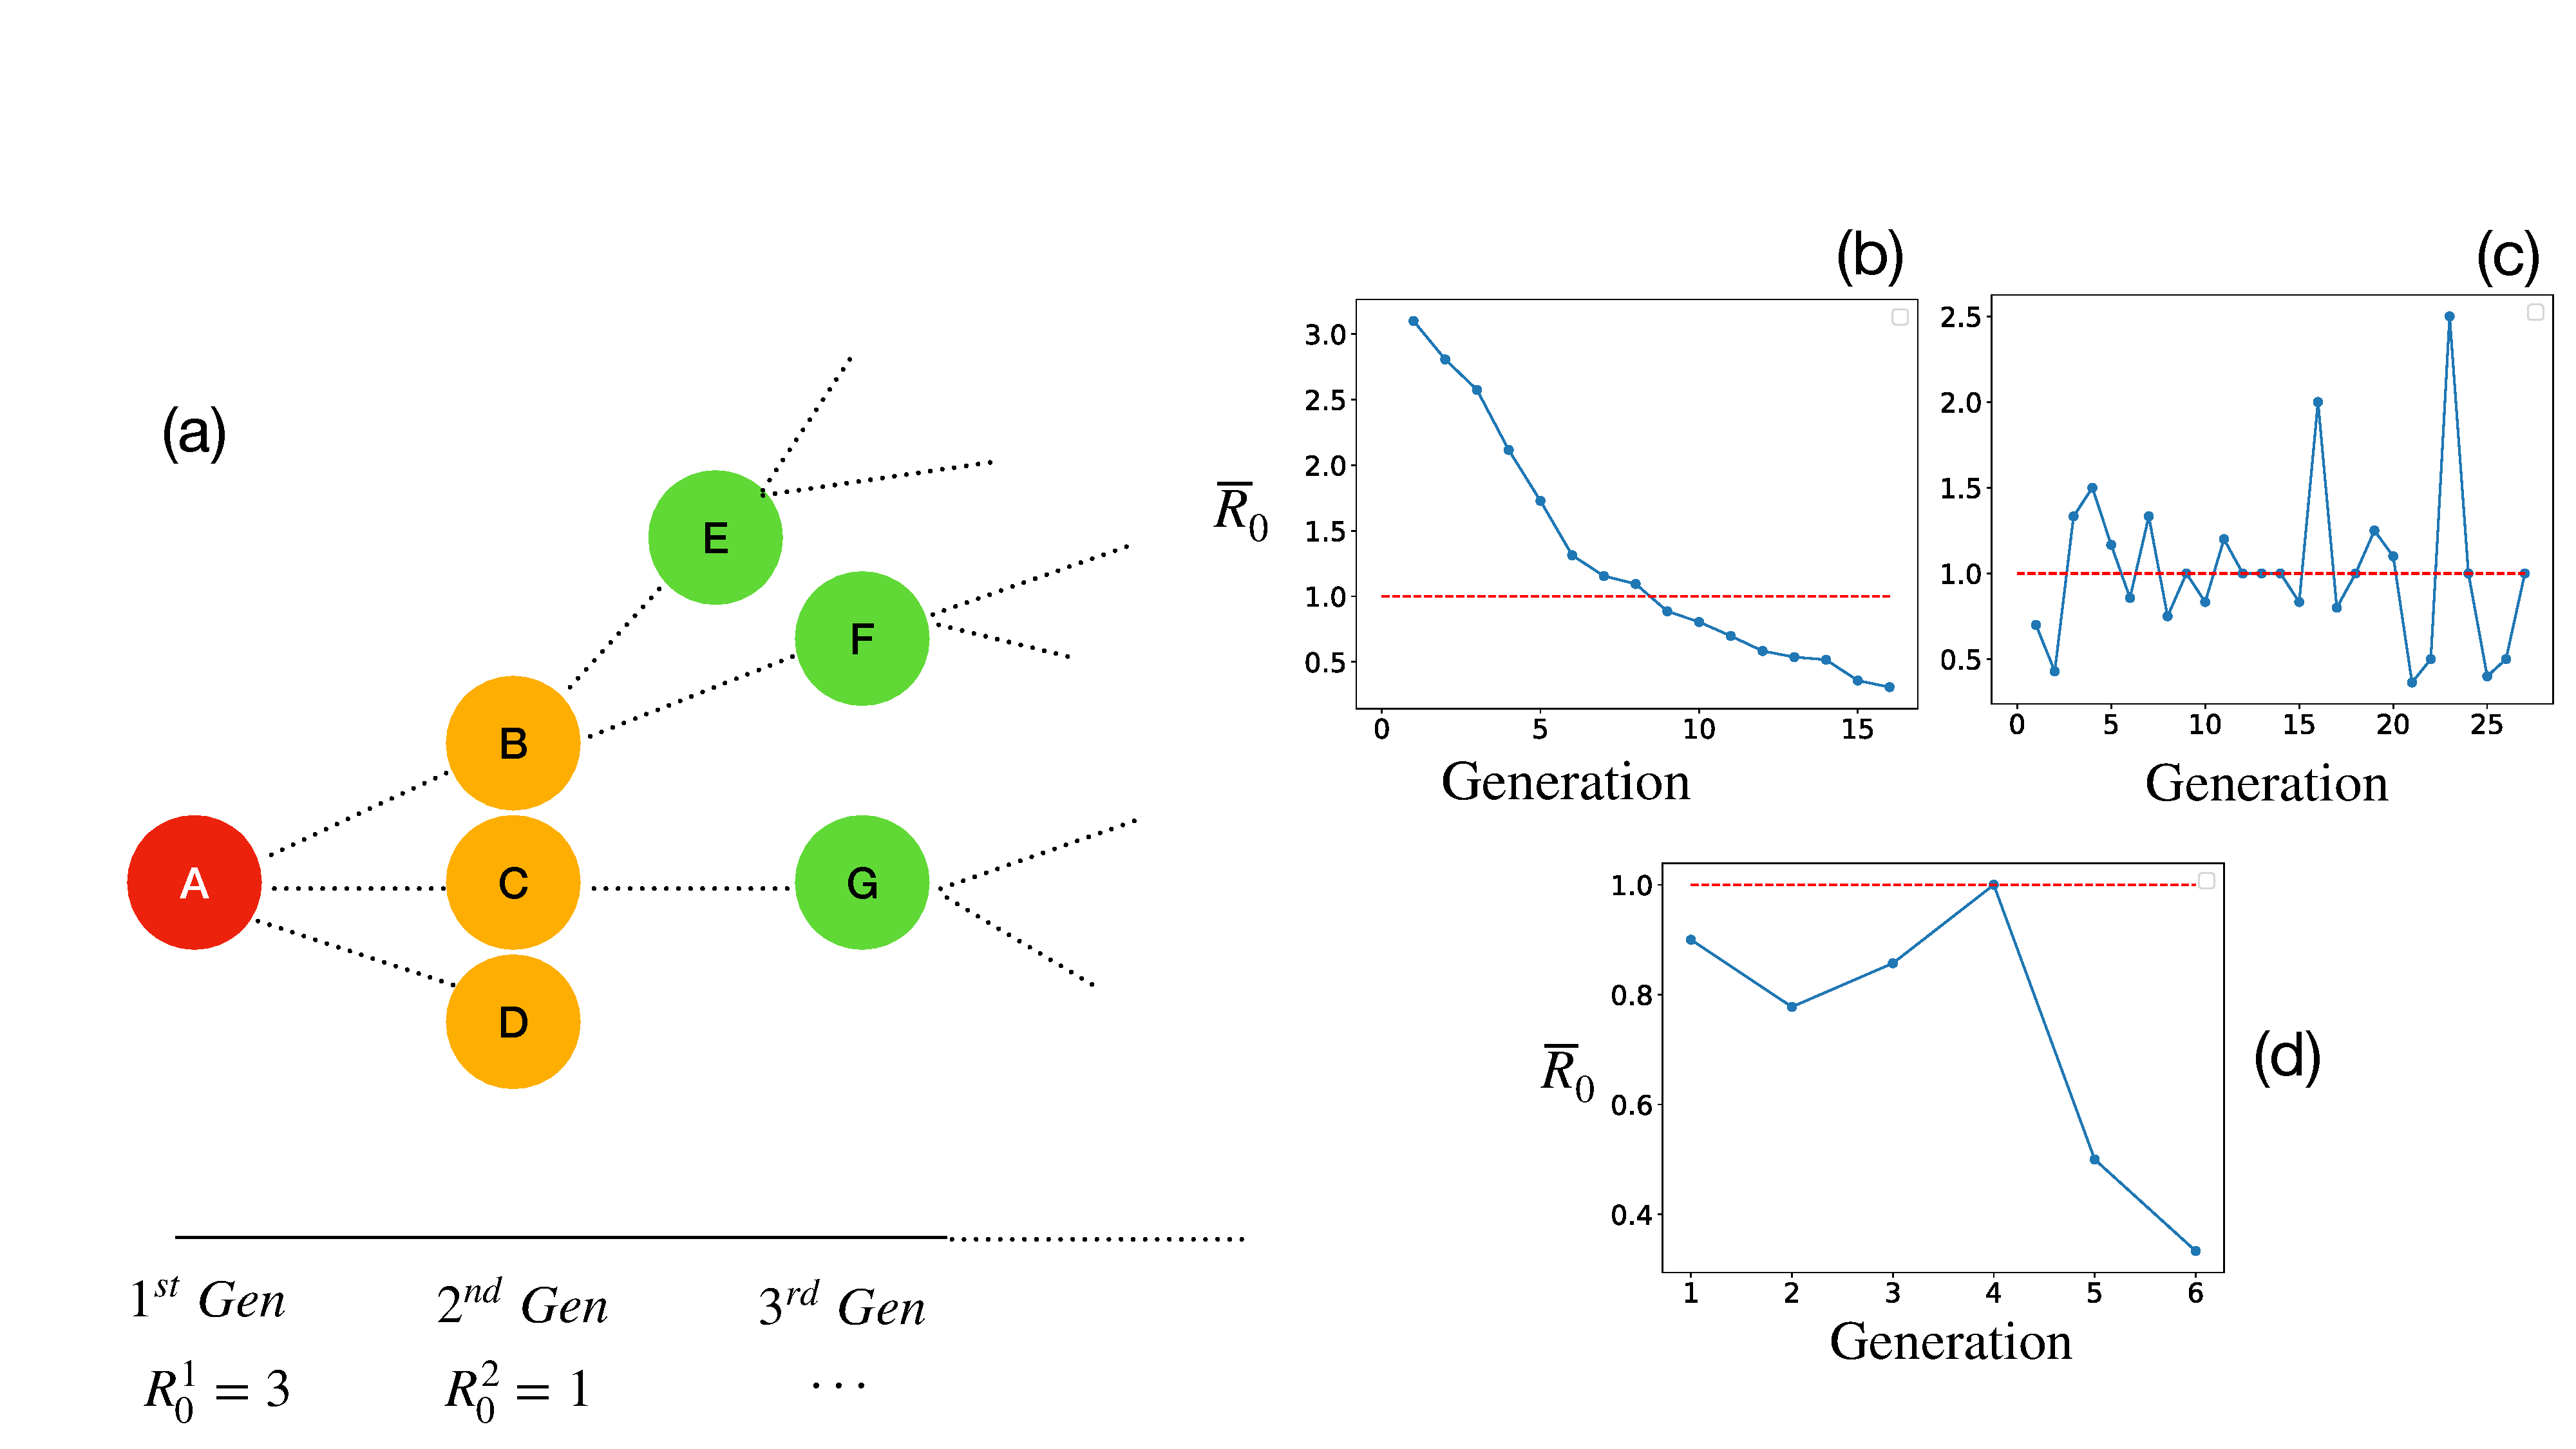
\includegraphics[scale=0.255]{chapter5/figures/fig1.pdf}
    \caption{Contact-traced $R_0$, the 'true' $R_0$. Tracking the history of all infected trees allows us to count how many infections are produced for each infectious tree over a simulation. At $t=0$, a single ($1^{st}$-generation) infection is positioned at the center of the domain. The quantity $R^i_0$ is defined as the mean number of infections produced for  the $i^{th}$ generation.}
    \label{fig:contact-trace}
\end{figure}

\subsection{Capturing $R_0$ in space and time}

In Figure \ref{fig:contact-trace}(b), we can see that measuring $R_0$ in a typical simulation, %
will likely over-estimate the contagiousness of the pathosystem at earlier times. %
Whereas, if $R_0$ is measured for later times (and the pathogen is above threshold), an %
under-estimate of the pathosystem contagiousness is likely. %
This is intuitive because the density of susceptible neighbors is higher at earlier times, %
on account of the neighborhood being untouched by other infected trees. %
The converse is true for later times in the simulation producing under-estimates. %
The number of secondary-infected trees will thus vary over time\footnote{Variations can %
also be expected at different locations through the domain. That is, centrally-distributed %
trees would, in theory, have access to infected more susceptible neighboring than trees %
located on the edge of the domain.}. %

Figure \ref{fig:contact-trace}(c) reveals how the pathosystem can behave if the threshold for %
invasion is just satisfied. %
Here $R_0$ is just above threshold for earlier times and barely spreads, however, the spread is chaotic. %
This can be considered a non-local generalisation of the SLM spreading on the critical point. %
In this scenario, $R_0$ is not strongly dependant on time. %
In the below-threshold regime, $R_0$ remains below $1$ for all generations and dies out after %
two generations. %

From Figures \ref{fig:contact-trace}(b-d), we have demonstrated that this definition of $R_0$ %
reliably captures the threshold of transmission during the initial stage of infection. %
Undesirably, we have made simplification in the assumptions and have not achieved a complete %
characterisation of $R_0$\textemdash which could, in be defined in terms of a growth %
rate per generation \cite{R0-construct}. %

We have not considered the re-growth of susceptible trees. %
If the number of susceptible hosts is fixed, without replacement, the number of susceptible hosts %
will continually decrease in time if an epidemic takes hold. %
This will reduce $R_0$ drastically for later time-periods. %
It appears inescapable that tree and plant-based systems violate the well-mixed population %
assumption that classic definitions of $R_0$ are based on. %
\textcolor{red}{Investigate how the next generation operator is used in the literature.}\\

% Averaging R0 over the entire ensemble will reduce R0, thus flatten the R0 map and reduce the amount of spatial clustering we see -- could illustrate this with a figure.

\subsection{$R_0$ and spatial scale}

Given that we have now defined $R_0$, we will investigate how this quantity changes in relation %
to the parameters dictating the spatial scale in our model. %
The parameters of interest are domain size $L$ and scale parameter $\alpha$. %
The domain size $L$ controls the array dimension stored in  memory, while $\alpha$ %
describes the physical space per-point inside the array i.e. the model resolution. %
The number of infections produced for each generation, $R_0^i$, were ensemble averaged with %
different values of domain size $L$ and scale parameter $\alpha$, %
shown in Figure \ref{fig:R0-spatial-scale}. Simulations started with a single infected, %
primary source, tree at the center of the domain and continued until the primary source %
transitioned into $I\rightarrow R$. %
The final number of contact-traced secondary infections produced from the primary infection %
constitute $R_0$.\\

The scale parameter of $5\mathrm{m}$, together with $L$, describe a range of different modelled %
areas which could represent fields, forests, stands or patches of land etc\footnote{Throughout this chapter, %
we take the domain to represent the average density of trees through a landscape.}. %
In Figure \ref{fig:R0-spatial-scale}(a), we can see values of $R_0^i$ increase with $L$ and %
begin to saturate to constant levels with a domain size $L\times L=1000\times 1000$, or $5\mathrm{km}\times 5 \mathrm{km}$. %
Beyond which, changes in domain size had negligible effects on $R_0$. %
This suggests for domain-sizes, up to some limit, the invasiveness of the pathogen has a %
dependence on the domain-size within which we choose to measure the spread. %
The result of Figure \ref{fig:R0-spatial-scale}(a) falls nicely in line with the work of %
others \cite{mikaberidze2016invasiveness} and suggests that the spatial scale is likely to %
alter the threshold of invasion.\\

The result of Figure \ref{fig:R0-spatial-scale}(a) is intuitive. %
Suppose we decide to calculate $R_0$ for a \textit{small} patch of land at density $\rho$, %
given a number of infected trees. In the case of wind-dispersal, it is clear to see that some %
innoculum (e.g. spores) would disperse out of the patch of land and infect other trees in %
neighbouring patches we are not considering. The value of $R_0$ is therefore subject to %
under-estimation for domain sizes small in comparison to the scale of dispersal.\\ 

On the other hand, suppose we measure $R_0$ for a larger patch of land at the same density $\rho$. Here, it is clear to see that we would count more secondary infections per infected tree and therefore measure a higher value of $R_0$. That is, the majority of dispersed inoculum will now land inside the domain boundary and directly effect the trees we are considering. At some point increasing the domain size will have no effect on $R_0$. This is likely to occur when the amount of inoculum, produced per tree\footnote{In our case $\beta$ represents a simplified compound parameter incorporating the amount of spores produced per tree and the probability of spore uptake by another $S$-tree.}, saturates the domain with only negligible amount of dispersing out of the patch.\\

\begin{figure}
    \centering
    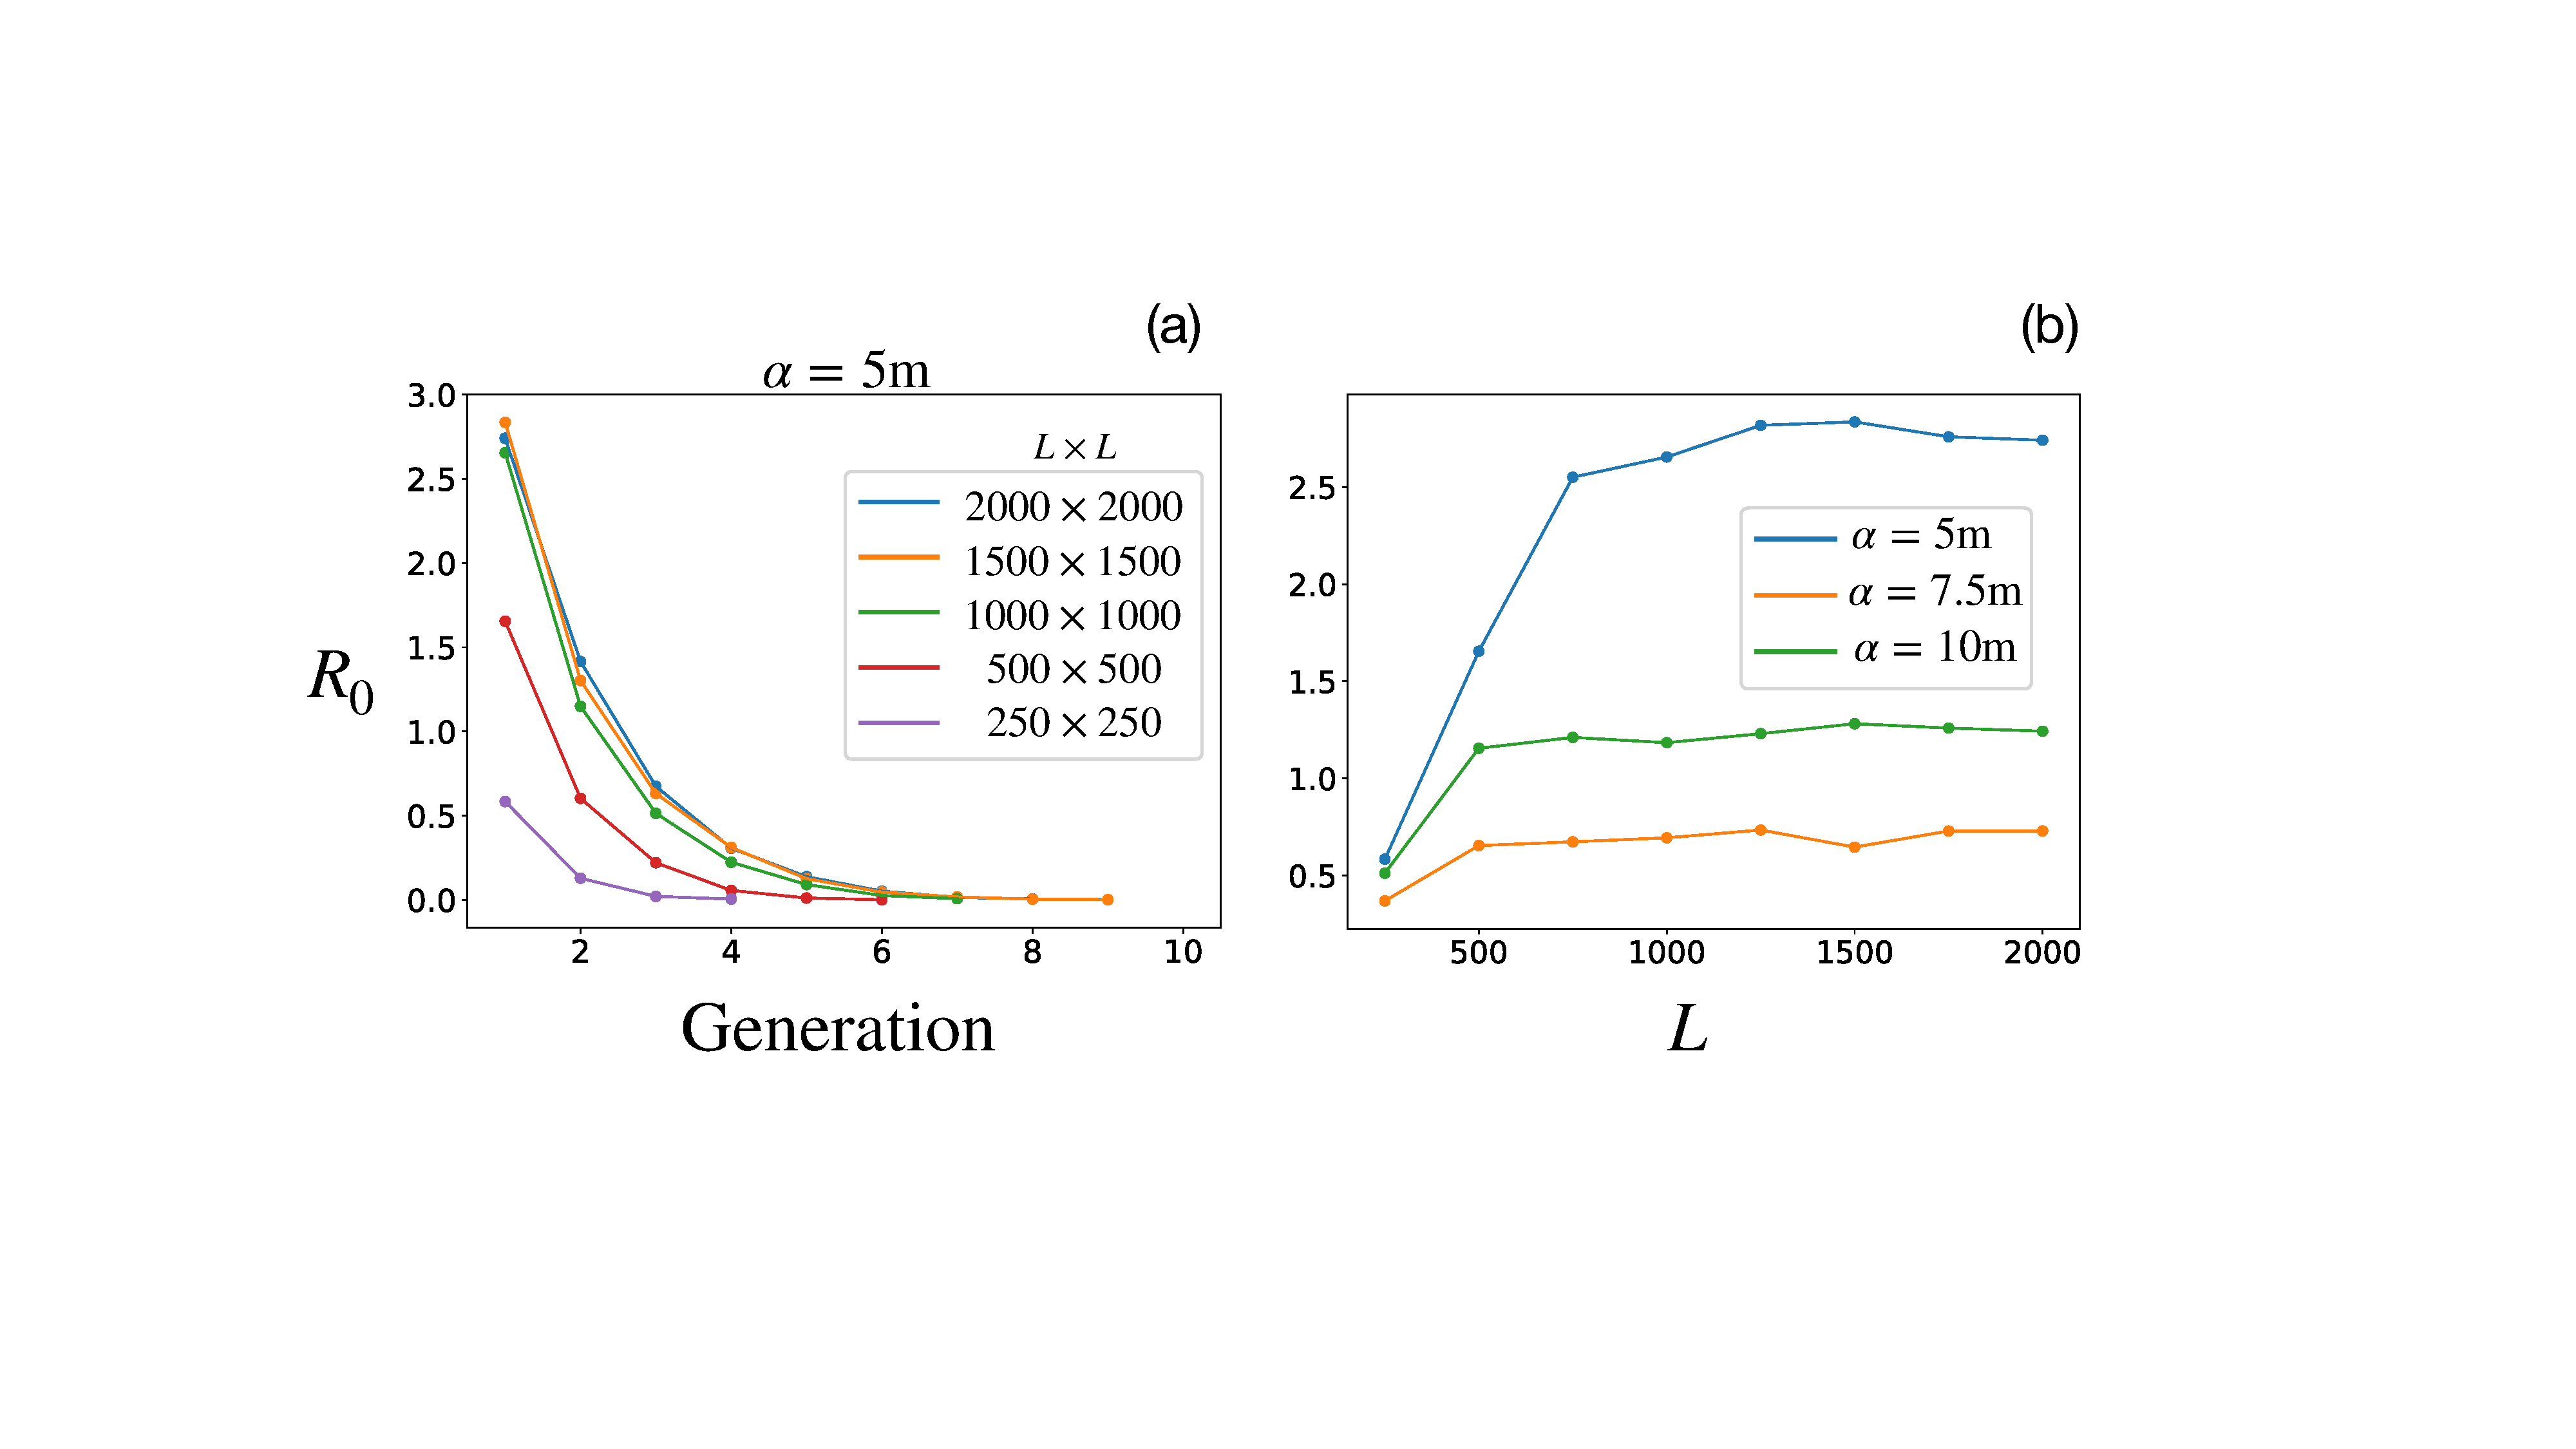
\includegraphics[scale=0.3]{chapter5/figures/fig2.pdf}
    \caption{How $R_0$ depends on scale...}
    \label{fig:R0-spatial-scale}
\end{figure}

Figure \ref{fig:R0-spatial-scale}(b) shows the model behaviour when the scale parameter is %
changed in conjunction with the domain size $L$. From this we notice a drastic and surprising %
reduction in the scale of pathogen spread for higher $\alpha$. %
This points towards a limitation in our model infectivity parameter $\beta$. %
Increasing $\alpha$ has the effect of increasing the average spacing between trees and %
increasing effective host canopy cover. %
In changing $\alpha$, the spatial resolution is rescaled and the expectation is that a higher value of $\beta$ should be seen to reflected a larger canopy cover. %
The infectivity $\beta$ represents a simplified compound parameter that incorporates information about the spore production rate. %
Re-scaling the canopy cover means more susceptible plant material can become infected and produce further spores. 
% JS_what does this mean 
\textcolor{red}{Tighten me up, talk about me to group.}\\

% beta is a per-capita rate of infection, that can be seen as a compound parameter...